\documentclass[11pt]{article}
\usepackage[left=1in,right=1in,top=0.75in,bottom=0.75in]{geometry}
\usepackage{amsmath}
\usepackage{graphicx}
\usepackage{float}
\usepackage[hidelinks]{hyperref}
\usepackage{microtype}
\setlength{\intextsep}{6pt plus 1pt minus 1pt}
\setlength{\abovecaptionskip}{5pt}

\begin{document}

Here is what I have worked on and the roadmap:

\subsubsection*{Paper I: ADAPT-VQE Ground State}
My algorithm ranks operators ($A$) by energy per cost $\Delta E(A)/K(A)$ within a position $p$ of the current ansatz circuit $U(\theta)$. I write the pair as
\[
r=(A,p) \mapsto e^{i\alpha A} \mapsto U(\theta)|\phi_{\rm ref}\rangle=|\psi\rangle.
\]

\textit{Main novelty:}

- Shortlisting of the operator set to obtain higher-order energy modeling while using fewer quantum measurements than scoring or modeling the full operator set.

- Scoring operators per unit hardware cost.

- An operator-pool definition for the Hubbard--Holstein model with high relevance to physical response channels.

\textit{Minor novelties:}

- An energy model for adding multiple operators at once, an energy model for deleting an operator from $U(\theta)$, and the first application of Lowerre-style beam search to ADAPT-VQE.

- Fubini--Study metric treatment. This enables trust-region-based modeling to keep the model local on the manifold and coordinate whitening to produce an orthonormal basis on the retained non-null tangent support, which helps inner optimization procedures and reduces the required quantum measurements.

I am still interested in making minor algorithm changes to improve the results comparison, although I think the current results are already strong.


\subsubsection*{Paper II: Time Dynamics of Hubbard--Holstein}
This paper time-evolves a Paper-I ground-state ansatz with the McLachlan variational principle. It relies on Fubini--Study metric Gram-matrix inversion and classical-computer-side ODE integration.

\textit{Novelty/contribution:}

- Ablation of ansatz generators when they are scored as redundant. As in my ground-state ADAPT preparation, generators can be added and removed per unit cost. I have not seen prior work that removes or ablates generators during McLachlan propagation.

- Quantum-algorithm simulation of a driven Hubbard--Holstein system.

- Possible numerical-stabilization improvements.

\textbf{PRELIMINARY RESULTS:}

Figure~\ref{fig:paper-ii-results} uses an ansatz purposefully made redundant and bloated with operators. This makes the Gram-matrix inversion more difficult because of null directions and makes the stabilization and pruning tests more informative. For this one case, the reductions relative to fixed McLachlan are shown below. The energy and doublon percentages are reductions in the final-time absolute error at $t=5\,t_{\rm hop}^{-1}$ relative to exact propagation from the same ADAPT-VQE seed state.

\begin{center}
\small
\begin{tabular}{lrrrr}
\hline
Method & \shortstack{Final-time\\energy-error reduction} & \shortstack{Final-time\\doublon-error reduction} & \shortstack{Parameter\\reduction} & \shortstack{$N_{2q}$\\reduction} \\
\hline
Stabilization & $14.5\%$ & $47.9\%$ & $0\%$ & $0\%$ \\
Stabilization + pruning & $37.0\%$ & $70.3\%$ & $24.6\%$ & $33.0\%$ \\
\hline
\end{tabular}
\end{center}

\begin{figure}[H]
    \centering
    \small\textbf{Legend:} Hubbard--Holstein dimer with Gaussian drive ($A=0.8$) and a time grid through $t=5\,t_{\rm hop}^{-1}$. Blue: McLachlan propagation, with stabilization and pruning status indicated by each plot title; orange: exact propagation from the exact ground state; green: exact propagation from the ADAPT-VQE ground state; pale vertical bands: numerical stabilization active; red diamonds: accepted generator ablations.
    \par\medskip
    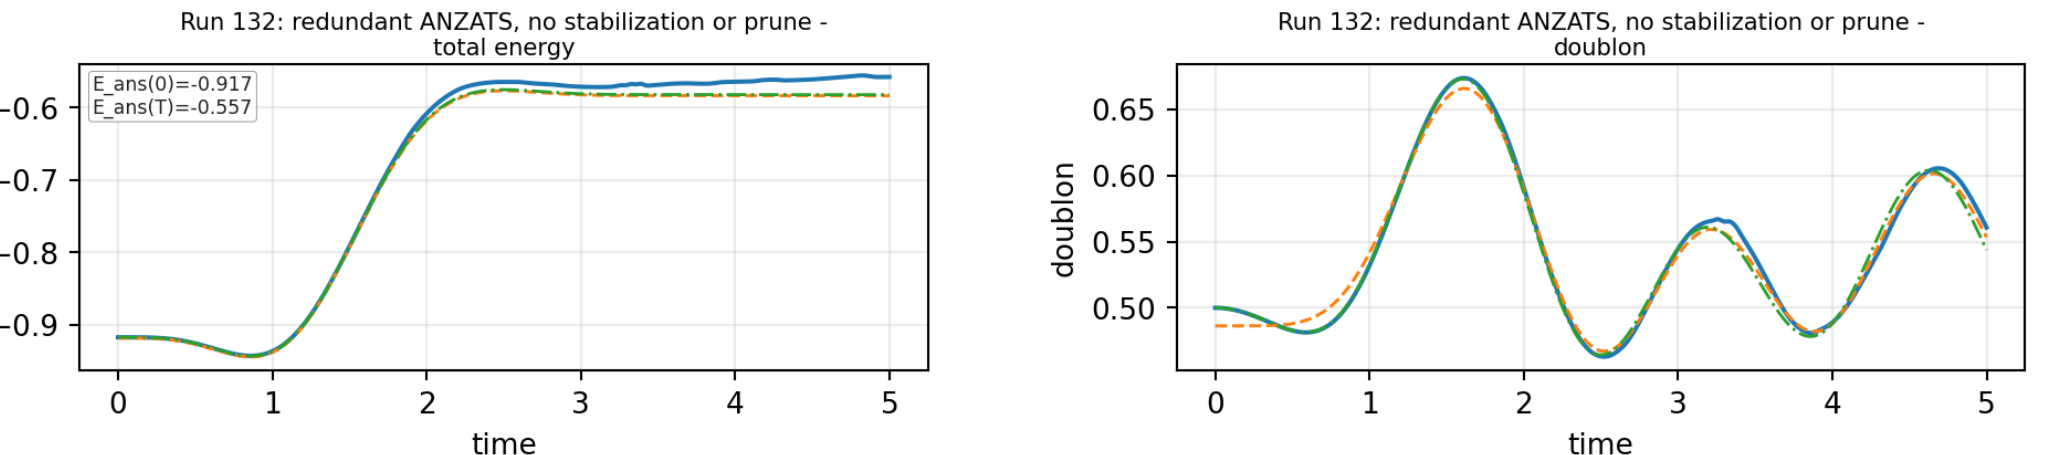
\includegraphics[width=0.80\linewidth]{advisor_project_overview_assets/results_pdf_crops/run132_fixed_energy_doublon.png}
    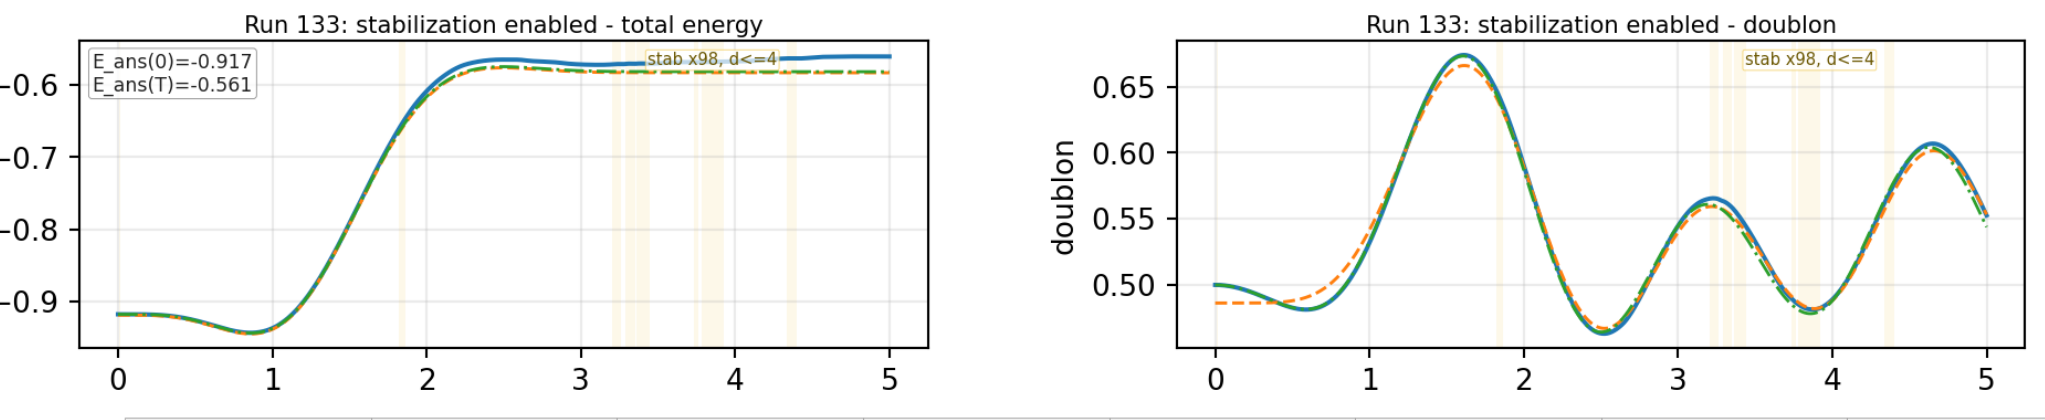
\includegraphics[width=0.80\linewidth]{advisor_project_overview_assets/results_pdf_crops/run133_stabilization_energy_doublon.png}
    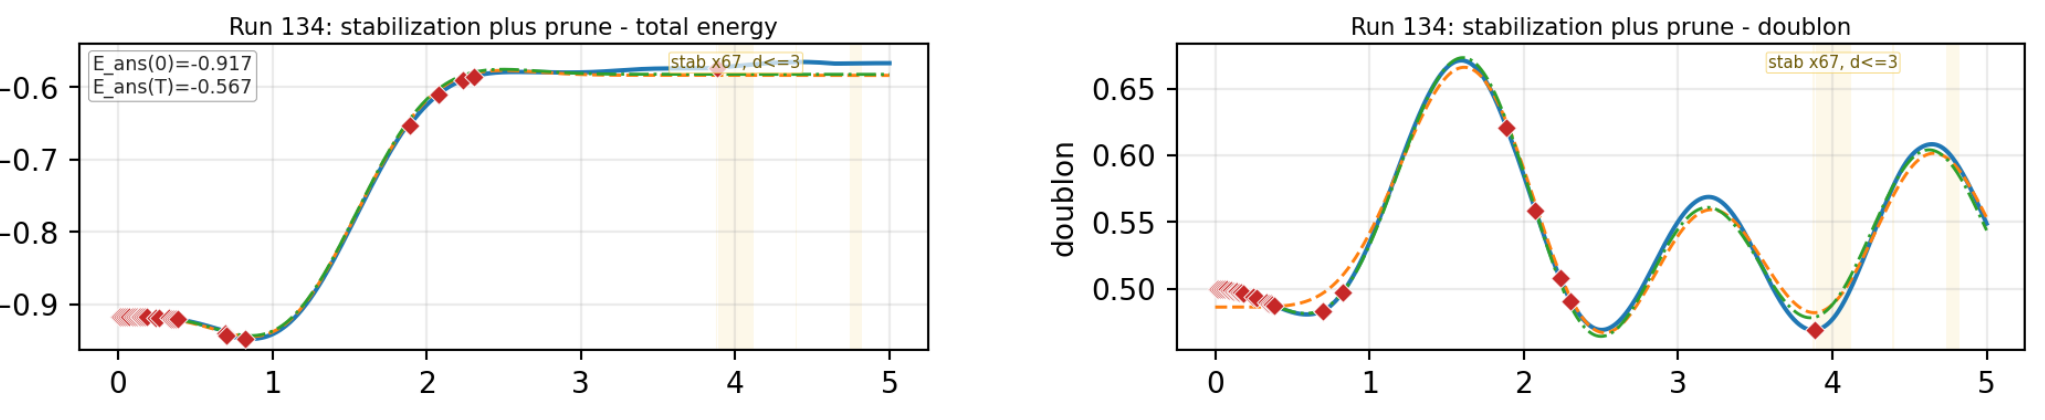
\includegraphics[width=0.80\linewidth]{advisor_project_overview_assets/results_pdf_crops/run134_stabilization_prune_energy_doublon.png}
    \caption{Total-energy and doublon trajectories: fixed McLachlan (top), numerical stabilization (middle), and numerical stabilization with pruning (bottom).}
    \label{fig:paper-ii-results}
\end{figure}

\subsubsection*{Paper III: Quantum Subspace Expansion (QSE) and Excited-State Dynamics}
This paper also uses the Paper I and II methods. It starts from the ground-state preparation ansatz, finds excited states, and performs time dynamics on these states. It uses the same physically motivated operators to construct a basis consisting of candidate excitation directions. The Hamiltonian is then projected into this excitation manifold and solved through a generalized Rayleigh--Ritz eigenvalue problem to obtain excitation states and transition strengths. The numerical-stabilization machinery used in Papers I and II to control ill-conditioning also applies here. As usual, we can rank operator-basis construction per unit hardware cost, and possibly my ``novelty'' multiplication factor from an older Paper I version will return for this basis construction.

\textit{Novelty:}

- The Paper I and II methods.

- The Hubbard--Holstein model and electron--phonon systems.

- Basis-per-unit-cost construction.

- Greater use of Hubbard--Holstein physical structure.

Again using the Hubbard--Holstein dimer, QSE reproduces the first-excitation gap ($0.865200327$, versus the exact reference $0.865200264$) with state fidelity $0.999999983$. Figure~\ref{fig:paper-iii-gap-spectrum} shows the matched excited-state gaps. Figure~\ref{fig:paper-iii-promoted-ap} compares the Paper II AP-McLachlan method against fixed McLachlan. Paper II adds generators, which is not itself novel, whereas fixed McLachlan does not; adding operators during dynamics is necessary for accuracy in this example.

\begin{figure}[H]
    \centering
    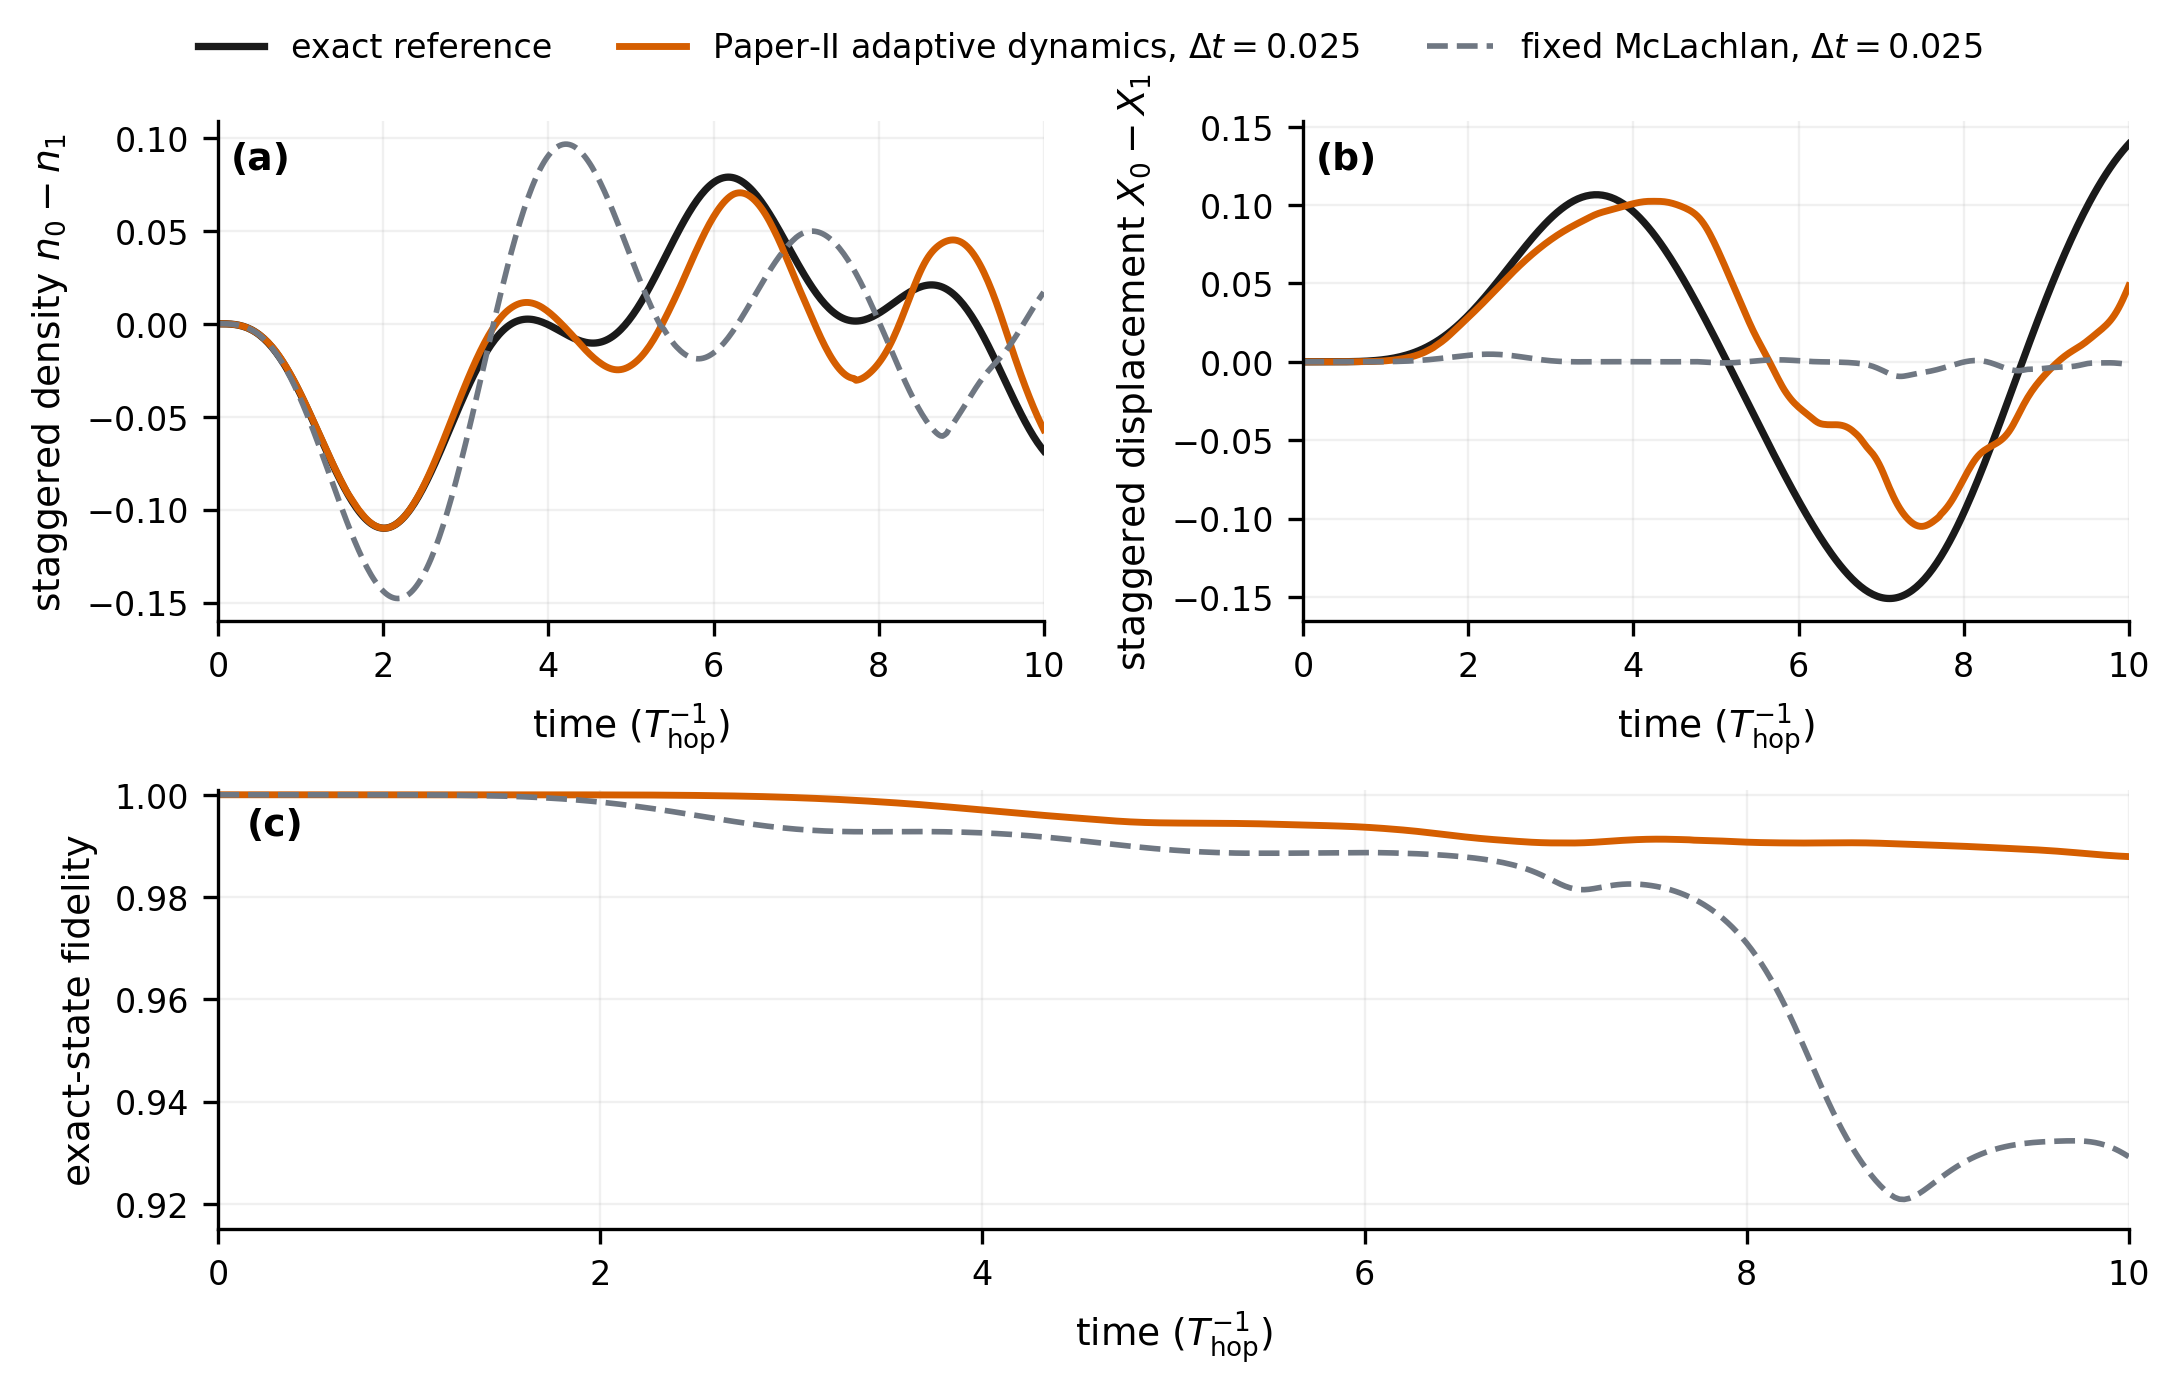
\includegraphics[width=0.78\linewidth]{advisor_project_overview_assets/paper_iii/paper_iii_promoted_ap_diagnostic.pdf}
    \caption{\textbf{BLACK = EXACT; ORANGE = PAPER-II ADAPTIVE DYNAMICS; DASHED GRAY = FIXED MCLACHLAN.} FIRST QSE EXCITED STATE. MINIMUM FIDELITY = \(0.9879\) (ADAPTIVE), \(0.9209\) (FIXED).}
    \label{fig:paper-iii-promoted-ap}
\end{figure}

\begin{figure}[H]
    \centering
    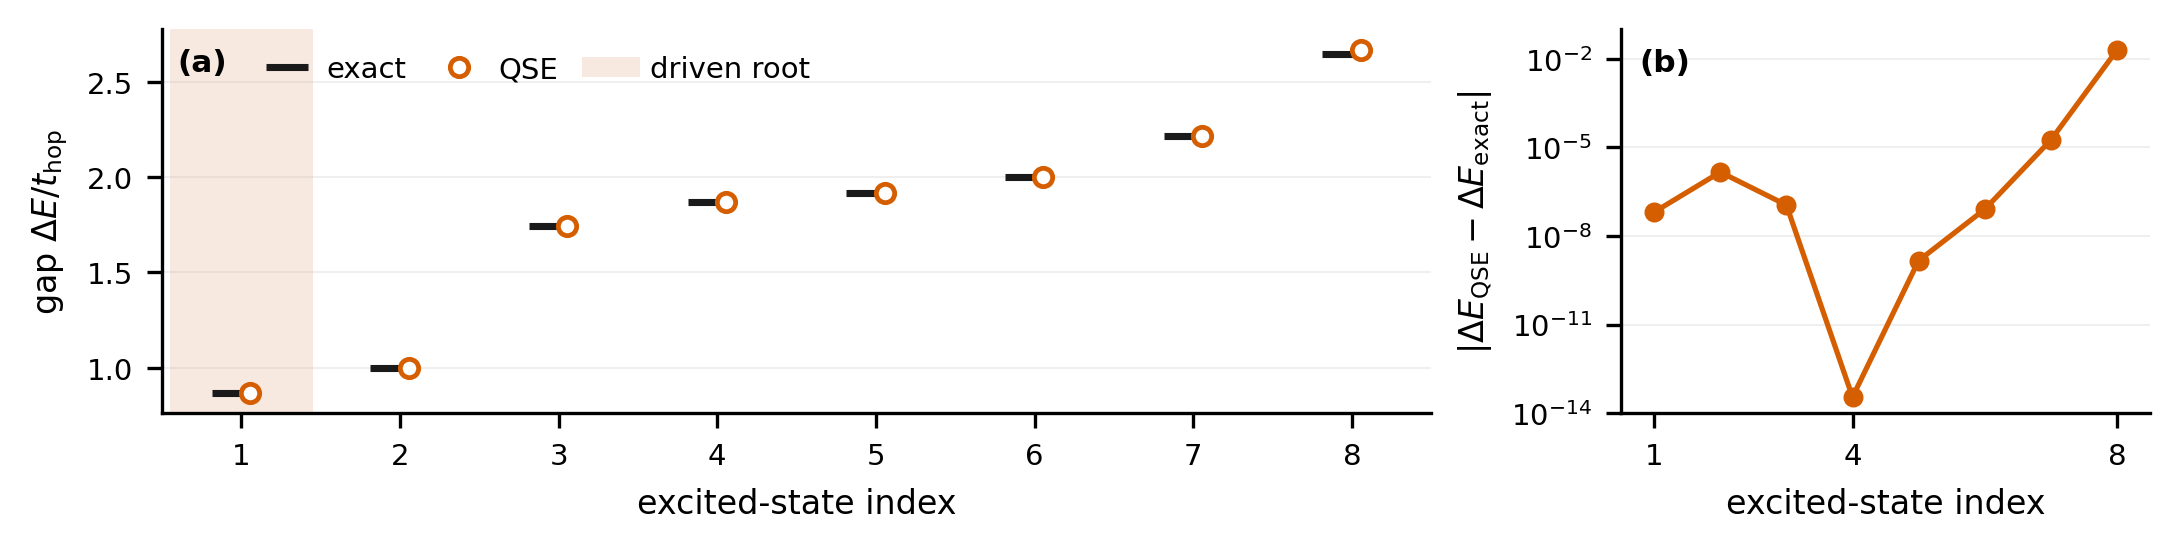
\includegraphics[width=0.78\linewidth]{advisor_project_overview_assets/paper_iii/paper_iii_qse_gap_spectrum.pdf}
    \caption{QSE EXCITED-STATE GAPS. (a) EXACT VS QSE; SHADED = STATE USED IN FIG.~\ref{fig:paper-iii-promoted-ap}. (b) ABSOLUTE GAP ERROR. IDEAL-STATEVECTOR DIAGNOSTIC.}
    \label{fig:paper-iii-gap-spectrum}
\end{figure}

\subsubsection*{Paper IV: From Molecular Vibronics to Periodic Materials}
Paper IV applies Papers I--III to first-principles electron--vibration Hamiltonians, a direction Jacopo proposed.

\textbf{Completed H$_2$O validation.} I computed the equilibrium electronic structure and all three harmonic modes---bend, symmetric stretch, and antisymmetric stretch---with Psi4. PySCF reproduces the Psi4 energy and frequencies at the same geometry; I also reproduce Doron's values at his geometry.

\textbf{Novelty:} The H$_2$O model uses an 8-electron/6-orbital active space and quantizes all three modes. Its coupling matrices are central differences of the electronic Hamiltonian along each mode after orbital alignment. Paper I prepares the ground state, Paper III computes vibronic excited states, and Paper II propagates the response to a kick. The next molecule is a small chiral system whose angular-momentum response spectrum will be computed after a kick pulse.

\textbf{Periodic extension.} Electrons \(\rightarrow\) phonons \(\rightarrow\) embedded Hamiltonian \(\rightarrow\) qubit estimate. A tungsten calculation is underway. Quantum ESPRESSO/DFPT/EPW will provide Bloch states, selected phonons, and electron--phonon matrix elements in a \(k\)-point plane-wave basis. \href{https://doi.org/10.1038/s41524-020-00353-z}{Quantum embedding} will produce a small active Hamiltonian, checked with PySCF-PBC. Papers I--III connect this Hamiltonian to the group's density-matrix and neutron-scattering work.

\clearpage
\subsubsection*{Paper V: Quantum Integration of the Non-Markovian Electron--Phonon EOM}
Paper V will develop a quantum algorithm for integrating the matrix equations of motion in the group's \href{https://arxiv.org/abs/2606.22233}{non-Markovian electron--phonon work}.

\textbf{Additional result for the group.} Gabriele's group-meeting slides showed that the archived matrix EOM diverges in the dimer test at \(\lambda=1.5\). Here \(\lambda=2g^2/(t_{\mathrm{hop}}\omega_{\mathrm{ph}})=2E_{\mathrm p}/t_{\mathrm{hop}}\), with \(E_{\mathrm p}=g^2/\omega_{\mathrm{ph}}\). For the dimer, \(\lambda=1.5\) lies above the mean-field bifurcation at \(\lambda=1\), on the localized, lattice-dressed branch; it is a finite-system stress point, not an exact quantum phase transition.

I used an affine Bloch decomposition to rewrite the archived matrices as a minimal vector of 31 independent real coordinates for the electron density, phonon moments, and electron--phonon correlations. Matrix positivity and trace define the physical region and reveal when the EOM velocity would drive a matrix away from positive semidefiniteness.

At every integration stage, I add the smallest correction to the 31-coordinate velocity that enforces the matrix and trace constraints while conserving energy. This prevents the \(\lambda=1.5\) divergence through \(t=1000\,t_{\mathrm{hop}}^{-1}\), although observable accuracy at this same point remains poor (Fig.~\ref{fig:paper-v-observables}).

I then tested whether higher-order moments fix the remaining error. In an offline exact-state test, supplying the missing higher-order correlations reduces the local derivative error from \(0.167\) to \(2.5\times10^{-5}\); these correlations are not inputs to the corrected propagation. Complete third- and fourth-order tests (47 and 82 coordinates) improve the lower-order equations but shift the main error to the newly added highest-order moment. I am now looking for a physical closure that also improves the observables at \(\lambda=1.5\).

\begin{figure}[H]
    \centering
    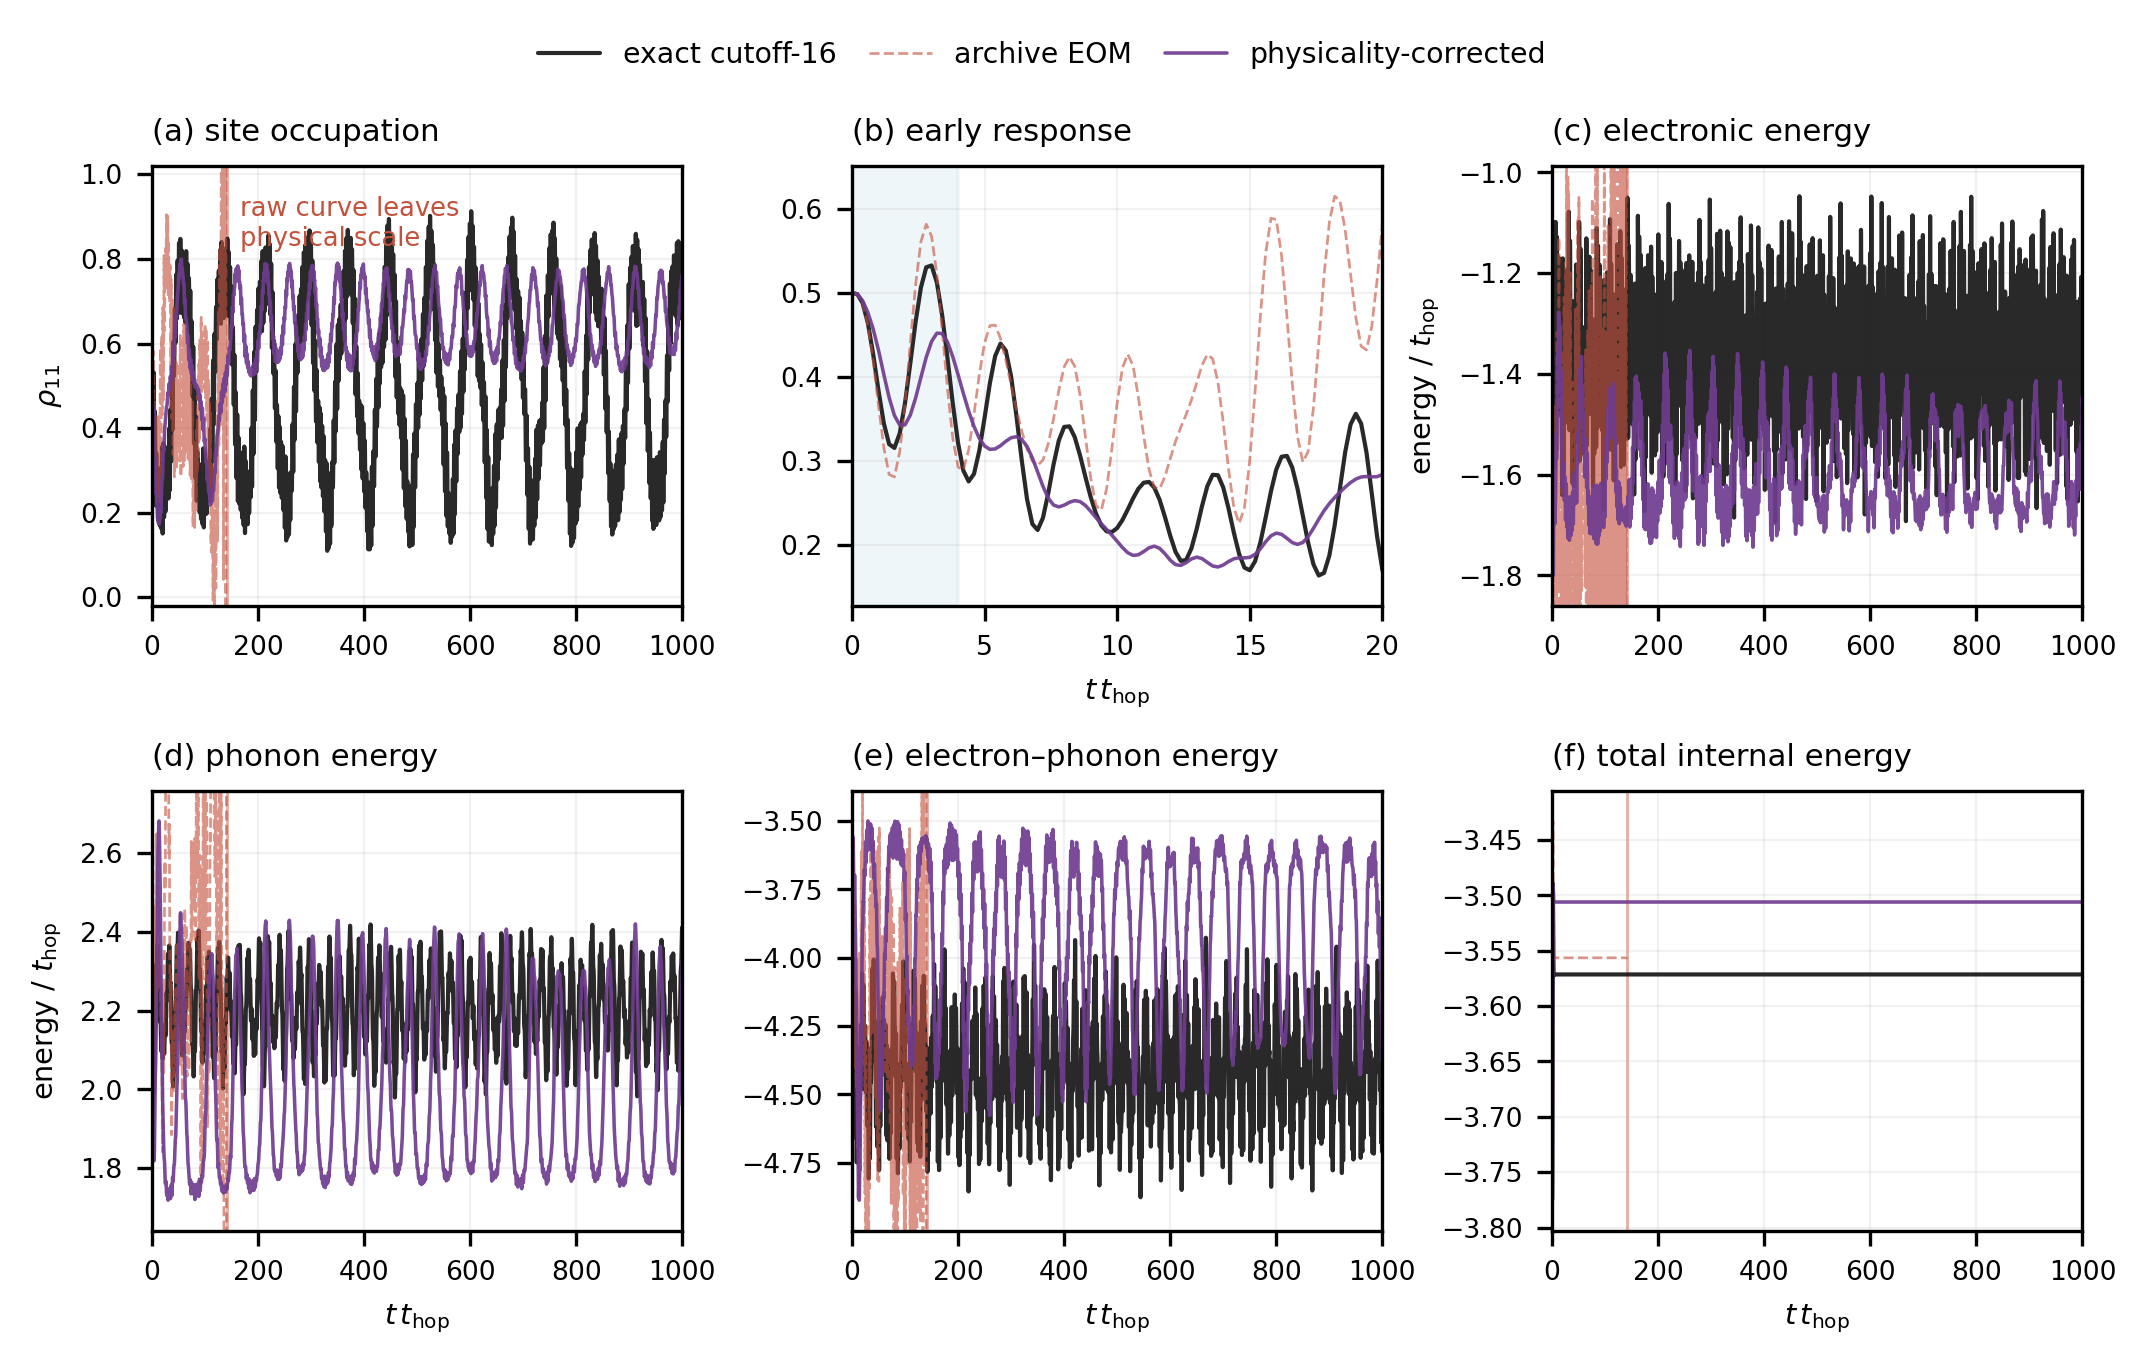
\includegraphics[width=\linewidth]{advisor_project_overview_assets/paper_v/paper_v_archive_observable_trajectories.pdf}
    \caption{\textbf{\(\lambda=1.5\): BLACK = EXACT; DASHED RED = ARCHIVE EOM; SOLID PURPLE = CORRECTED ARCHIVE EOM.} DIVERGENCE REMOVED THROUGH \(t=1000\,t_{\mathrm{hop}}^{-1}\); OBSERVABLE ERROR REMAINS.}
    \label{fig:paper-v-observables}
\end{figure}

\begin{figure}[H]
    \centering
    \footnotesize
    \textbf{(a) PHYSICALITY}\par\vspace{2pt}
    \includegraphics[width=0.50\linewidth]{advisor_project_overview_assets/paper_v/paper_v_physicality_correction.pdf}

    \vspace{4pt}
    \textbf{(b) MISSING CORRELATIONS}\par\vspace{2pt}
    \includegraphics[width=0.72\linewidth]{advisor_project_overview_assets/paper_v/paper_v_missing_physics.pdf}

    \vspace{4pt}
    \textbf{(c) CORRECTION}\par\vspace{2pt}
    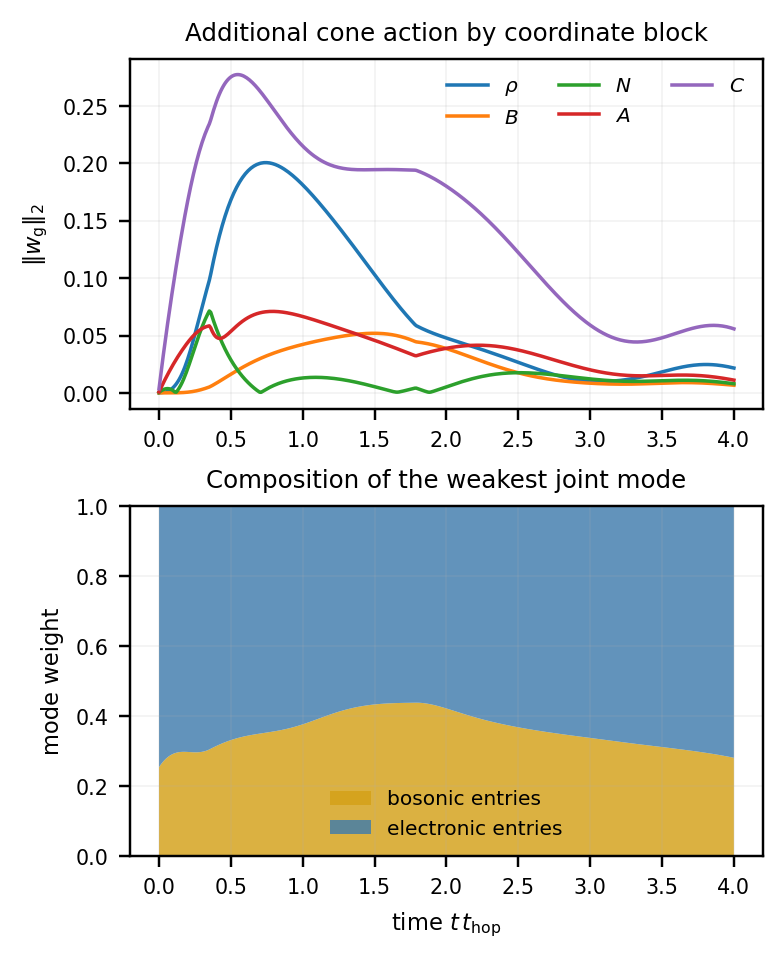
\includegraphics[width=0.34\linewidth]{MATH/paper_facing/paper_V_high_u_gkba/pedagogical/figures/joint_electron_phonon_mechanism_evidence.png}

    \small
    \caption{(a) RED = ARCHIVE EOM; BLUE = EXACT; GREEN = CORRECTED EOM. (b) LOCAL CORRELATION-EQUATION ERROR: BLUE = ARCHIVE; ORANGE/GREEN/RED = SUCCESSIVE MISSING HIGHER-ORDER CORRELATIONS. (c) CORRECTION BY MOMENT BLOCK; ELECTRON/PHONON CONTENT OF THE LIMITING MODE.}
    \label{fig:paper-v-support}
\end{figure}

\end{document}
